\bta{光的反射和折射}


\begin{enumerate}
	%\renewcommand{\labelenumi}{\arabic{enumi}.}
	% A(\Alph) a(\alph) I(\Roman) i(\roman) 1(\arabic)
	%设定全局标号series=example	%引用全局变量resume=example
	%[topsep=-0.3em,parsep=-0.3em,itemsep=-0.3em,partopsep=-0.3em]
	%可使用leftmargin调整列表环境左边的空白长度 [leftmargin=0em]
	\item
\exwhere{$ 2017 $ 年北京卷}
 如图所示,一束可见光穿过平行玻璃砖后,变为
$ a $、$ b $ 两束单色光。如果光束 $ b $ 是蓝光,则光束 $ a $ 可能是 \xzanswer{D} 
\begin{figure}[h!]
	\centering
	\includesvg[width=0.23\linewidth]{picture/svg/GZ-3-tiyou-1430}
\end{figure}

\fourchoices
{红光}
{黄光}
{绿光}
{紫光}




\item 
\exwhere{$ 2016 $ 年上海卷}
一束单色光由空气进入水中,则该光在空气和水中传播时 \xzanswer{D} 

\fourchoices
{速度相同,波长相同}
{速度不同,波长相同}
{速度相同,频率相同}
{速度不同,频率相同}




\item 
\exwhere{$ 2013 $ 年四川卷}
光射到两种不同介质的分界面,分析其后的传播情形可知 \xzanswer{D} 

\fourchoices
{折射现象的出现说明光是纵波}
{光总会分为反射光和折射光}
{折射光与入射光的传播方向总是不同的}
{发生折射是因为光在不同介质中的传播速度不同}


\item 
\exwhere{$ 2013 $ 年北京卷}
如图所示,一束可见光射向半圆形玻璃砖的圆心 $ O $,经折射后分为两束单色光 $ a $ 和 $ b $。下列判
断正确的是 \xzanswer{B} 
\begin{figure}[h!]
	\centering
	\includesvg[width=0.23\linewidth]{picture/svg/GZ-3-tiyou-1431}
\end{figure}

\fourchoices
{玻璃对 $ a $ 光的折射率小于对 $ b $ 光的折射率}
{$ a $ 光的频率大于 $ b $ 光的频率}
{在真空中 $ a $ 光的波长大于 $ b $ 光的波长}
{$ a $ 光光子能量小于 $ b $ 光光子能量}


\item 
\exwhere{$ 2013 $ 年福建卷}
一束由红、紫两色光组成的复色光,从空气斜射向玻璃三棱镜。下面四幅图中能正确表示该复
色光经三棱镜分离成两束单色光的是 \xzanswer{B} 

\pfourchoices
{\includesvg[width=4.3cm]{picture/svg/GZ-3-tiyou-1432}}
{\includesvg[width=4.3cm]{picture/svg/GZ-3-tiyou-1433}}
{\includesvg[width=4.3cm]{picture/svg/GZ-3-tiyou-1434}}
{\includesvg[width=4.3cm]{picture/svg/GZ-3-tiyou-1435}}


\item 
\exwhere{$ 2012 $ 年理综北京卷}
一束单色光经由空气射入玻璃,这束光的 \xzanswer{A} 


\fourchoices
{速度变慢,波长变短}
{速度不变,波长变短}
{频率增高,波长变长}
{频率不变,波长变长}



\item 
\exwhere{$ 2011 $ 年理综安徽卷}
实验表明,可见光通过三棱镜时各色光的折射率 $ n $ 随着波长 $ \lambda $ 的变化符合科西经验公式:
$n=A+\frac{B}{\lambda^{2}}+\frac{C}{\lambda^{4}}$
,其中 $ A $、$ B $、$ C $
是正的常量。太阳光进入三棱镜后
发生色散的情形如下图所示。则 \xzanswer{D} 
% TODO: \usepackage{graphicx} required
\begin{figure}[h!]
	\centering
\begin{subfigure}{0.4\linewidth}
	\centering
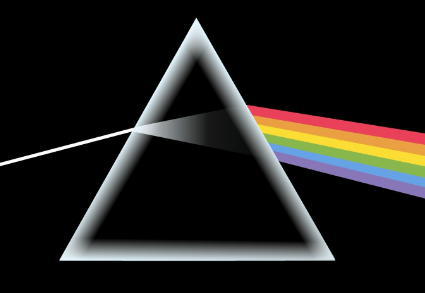
\includegraphics[width=0.7\linewidth]{picture/screenshot082}
	\caption{}\label{}
\end{subfigure}
\begin{subfigure}{0.4\linewidth}
	\centering
	\includesvg[width=0.7\linewidth]{picture/svg/GZ-3-tiyou-1436} 
	\caption{}\label{}
\end{subfigure}
\end{figure}

\fourchoices
{屏上 $ c $ 处是紫光}
{屏上 $ d $ 处是红光}
{屏上 $ b $ 处是紫光}
{屏上 $ a $ 处是红光}



\item
\exwhere{$ 2015 $ 年理综福建卷}
如图,一束光经玻璃三棱镜折射后分为两束单色光 $ a $、$ b $,波长分别为 $ \lambda_{a} $、
$ \lambda_{b} $,该玻璃对单色光 $ a $、$ b $ 的折射率分别为 $ n_{a} $、$ n_{b} $,则 \xzanswer{B} 
\begin{figure}[h!]
	\centering
	\includesvg[width=0.23\linewidth]{picture/svg/GZ-3-tiyou-1437}
\end{figure}


\fourchoices
{$\lambda_{a}<\lambda_{b}, \quad n_{a}>n_{b}$}
{$\lambda_{a}<\lambda_{b}, \quad n_{a}<n_{b}$}
{$\lambda_{a}>\lambda_{b}, \quad n_{a}<n_{b}$}
{$\lambda_{a}>\lambda_{b}, \quad n_{a}>n_{b}$}


\item 
\exwhere{$ 2015 $ 年理综四川卷}
 直线 $ P_{1} P_{2} $ 过均匀玻璃球球心 $ O $,细光束 $ a $、$ b $ 平行且关于 $ P_{1} P_{2} $ 对称,由空
气射入玻璃球的光路如图。$ a $、$ b $ 光相比 \xzanswer{C} 
\begin{figure}[h!]
	\centering
	\includesvg[width=0.23\linewidth]{picture/svg/GZ-3-tiyou-1438}
\end{figure}


\fourchoices
{玻璃对 $ a $ 光的折射率较大}
{玻璃对 $ a $ 光的临界角较小}
{$ b $ 光在玻璃中的传播速度较小}
{$ b $ 光在玻璃中的传播时间较短}



\item 
\exwhere{$ 2011 $ 年理综福建卷}
如图,半圆形玻璃砖置于光屏 $ PQ $ 的左下方。一束白光沿半径方向从 $ A $ 点射入玻璃砖,在 $ O $ 点
发生反射和折射,折射光在光屏上呈现七色光带。若入射点由 $ A $ 向 $ B $ 缓
慢移动,并保持白光沿半径方向入射到 $ O $ 点,观察到各色光在光屏上陆
续消失。在光带未完全消失之前,反射光的强度变化以及光屏上最先消
失的光分别是 \xzanswer{C} 
\begin{figure}[h!]
	\centering
	\includesvg[width=0.23\linewidth]{picture/svg/GZ-3-tiyou-1439}
\end{figure}

\fourchoices
{减弱,紫光}
{减弱,红光}
{增强,紫光}
{增强,红光}



\item 
\exwhere{$ 2011 $ 年理综全国卷}
雨后太阳光入射到水滴中发生色散而形成彩虹。设水滴是球形的,图中的圆代表水滴过球心的
截面,入射光线在过此截面的平面内,$ a $、$ b $、$ c $、$ d $ 代表四条不同颜色的出射光线,则它们可能依次
是 \xzanswer{B} 
\begin{figure}[h!]
	\centering
	\includesvg[width=0.23\linewidth]{picture/svg/GZ-3-tiyou-1440}
\end{figure}

\fourchoices
{紫光、黄光、蓝光和红光}
{紫光、蓝光、黄光和红光}
{红光、蓝光、黄光和紫光}
{红光、黄光、蓝光和紫光}


\item 
\exwhere{$ 2011 $ 年理综浙江卷}
“$ B $” 超”可用于探测人体内脏的病变状况。下图是超声波从肝脏表面入射,经折射与反射,最后从肝
脏表面射出的示意图。超声波在进入肝脏发生折射时遵循的规律与光的折射规律类似,可表述为
$\frac{\sin \theta_{1}}{\sin \theta_{2}}=\frac{v_{1}}{v_{2}}$(式中$ \theta_{1} $ 是入射角,$ \theta _{2} $ 是折射角,$ \nu_{1} $,$ \nu_{2} $ 为别是超声波在肝外和肝
内的传播速度)
,超声波在肿瘤表面发生反射时遵循的规律与光的反射规律相
同。已知$ \nu _{2} =0.9 \nu_{1} $,入射点与出射点之间的距离是 $ d $,入射角为 $ i $,肿瘤的反射
面恰好与肝脏表面平行,则肿瘤离肝脏表面的深度 $ h $ 为 \xzanswer{D} 
\begin{figure}[h!]
	\centering
	\includesvg[width=0.23\linewidth]{picture/svg/GZ-3-tiyou-1441}
\end{figure}


\fourchoices
{$\frac{9 d \sin i}{\sqrt{100-81 \sin ^{2} i}}$}
{$\frac{d \sqrt{81-100 \sin ^{2} i}}{100 \sin i}$}
{$\frac{d \sqrt{81-100 \sin ^{2} i}}{20 \sin i}$}
{$\frac{d \sqrt{100-81 \sin ^{2} i}}{18 \sin i}$}


\item 
\exwhere{$ 2011 $ 年理综四川卷}
下列说法正确的是 \xzanswer{A} 

\fourchoices
{甲乙在同一明亮空间,甲从平面镜中看见乙的眼睛时,乙一定能从镜中看见甲的眼睛}
{我们能从某位置通过固定的任意透明的介质看见另一侧的所有景物}
{可见光的传播速度总是大于电磁波的传播速度}
{在介质中光总是沿直线传播}



\item
\exwhere{$ 2014 $ 年理综北京卷}
以往,已知材料的折射率都为正值($ n>0 $)
。现已有针对某些电磁波设计制作的人工材料,其折
射率可以为负值($ n<0 $),称为负折射率材料。位于空气中的这类材料,入射角 $ i $ 与折射角 $ r $ 依然满
足$\frac{\sin i}{\sin r}=n$,但是折射线与入射线位于法线的同一侧(此时折射角取负值)。若该材料对于电磁 \xzanswer{B} 
\pfourchoices
{\includesvg[width=4.3cm]{picture/svg/GZ-3-tiyou-1442}}
{\includesvg[width=4.3cm]{picture/svg/GZ-3-tiyou-1443}}
{\includesvg[width=4.3cm]{picture/svg/GZ-3-tiyou-1444}}
{\includesvg[width=4.3cm]{picture/svg/GZ-3-tiyou-1445}}



\item 
\exwhere{$ 2019 $ 年物理天津卷}
如图为 $ a $、$ b $、$ c $ 三种光在同一光电效应装置中测的光电流和电压的关系。
由 $ a $、 $ b $、 $ c $ 组成的复色光通过三棱镜时,下述光路图中正确的是 \xzanswer{C} 
\begin{figure}[h!]
	\centering
	\includesvg[width=0.23\linewidth]{picture/svg/GZ-3-tiyou-1453}
\end{figure}

\pfourchoices
{\includesvg[width=4.3cm]{picture/svg/GZ-3-tiyou-1450}}
{\includesvg[width=4.3cm]{picture/svg/GZ-3-tiyou-1449}}
{\includesvg[width=4.3cm]{picture/svg/GZ-3-tiyou-1451}}
{\includesvg[width=4.3cm]{picture/svg/GZ-3-tiyou-1452}}


\item 
\exwhere{$ 2015 $ 年理综安徽卷}
 如图所示,一束单色光从空气入射到棱镜的 $ AB $ 面上,经 $ AB $ 和 $ AC $ 两个
面折射后从 $ AC $ 面进入空气。当出射角 $ i ^{\prime}  $ 和入射角 $ i $ 相等时,出射光线相对于入射光线偏转的角度
为$ \theta $。已知棱镜顶角为$ \alpha $,则计算棱镜对该色光的折射率表达式为 \xzanswer{A} 
\begin{figure}[h!]
	\centering
	\includesvg[width=0.23\linewidth]{picture/svg/GZ-3-tiyou-1454}
\end{figure}

\fourchoices
{$\frac{\sin \frac{\alpha+\theta}{2}}{\sin \frac{\alpha}{2}}$}
{$\frac{\sin \frac{\alpha+\theta}{2}}{\sin \frac{\theta}{2}}$}
{$\frac{\sin \theta}{\sin \left(\theta-\frac{\alpha}{2}\right)}$}
{$\frac{\sin \alpha}{\sin \left(\alpha-\frac{\theta}{2}\right)}$}





	
	
	
\end{enumerate}

